% =====================================================================
% Manual de usuario (Parte II de Manuales.tex)
% Responsable: Parte 6 — John Jairo Páez Albino
% Se incluye en Manuales.tex con % =====================================================================
% Manual de usuario (Parte II de Manuales.tex)
% Responsable: Parte 6 — John Jairo Páez Albino
% Se incluye en Manuales.tex con % =====================================================================
% Manual de usuario (Parte II de Manuales.tex)
% Responsable: Parte 6 — John Jairo Páez Albino
% Se incluye en Manuales.tex con % =====================================================================
% Manual de usuario (Parte II de Manuales.tex)
% Responsable: Parte 6 — John Jairo Páez Albino
% Se incluye en Manuales.tex con \input{secciones/manual-usuario.tex}.
% Usa los paquetes graphicx y booktabs, y las rutas son relativas a la
% raíz del repositorio.
% =====================================================================
\section{Manual de usuario}
\label{sec:manual-usuario}

Este manual explica, paso a paso, cómo correr una simulación, cómo correr todos los
escenarios del experimento, cómo generar las tablas y las gráficas y cómo leer los
resultados. La instalación de ns-3 y la estructura del código están en el manual
técnico.

\subsection{Antes de empezar}

Se necesita:

\begin{itemize}
    \item Ubuntu 22.04, nativo o en WSL2 sobre Windows.
    \item ns-3.43 compilado con los módulos \texttt{wifi}, \texttt{aodv},
    \texttt{mobility}, \texttt{internet}, \texttt{applications}, \texttt{flow-monitor}
    y \texttt{netanim} (ver el manual técnico).
    \item Python 3.10 o superior. Los scripts que corren y procesan las simulaciones solo
    usan la librería estándar; el de las gráficas necesita además \texttt{pandas},
    \texttt{matplotlib}, \texttt{scipy} y \texttt{numpy}.
    \item El repositorio del grupo, descargado en el disco de Linux (por ejemplo, en la
    carpeta personal \texttt{\textasciitilde}). En WSL no conviene trabajar en
    \texttt{/mnt/c/...}, porque compilar sobre el disco de Windows es mucho más lento.
\end{itemize}

\begin{verbatim}
cd ~
git clone https://github.com/10scar/tallerme01
cd tallerme01
python3 -m pip install pandas matplotlib scipy numpy
\end{verbatim}

En los ejemplos se supone que ns-3 está en \texttt{\textasciitilde/ns-allinone-3.43/ns-3.43}
y el repositorio en \texttt{\textasciitilde/tallerme01}; si están en otro lugar, basta
con cambiar esas rutas.

\subsection{Paso 1: correr una simulación}

El programa está en \texttt{simulacion/manet-jerarquica.cc}. ns-3 compila los programas
de su carpeta \texttt{scratch/}, así que primero se copia allí y luego se ejecuta desde
la carpeta de ns-3:

\begin{verbatim}
cp ~/tallerme01/simulacion/manet-jerarquica.cc ~/ns-allinone-3.43/ns-3.43/scratch/
cd ~/ns-allinone-3.43/ns-3.43
./ns3 run "scratch/manet-jerarquica --scenario=E3 --clusterSpeed=5 \
    --nodeSpeed=5 --simTime=200 --RngRun=1 \
    --outDir=$HOME/tallerme01/resultados/raw"
\end{verbatim}

La primera vez, \texttt{./ns3 run} compila el programa antes de ejecutarlo. Los
parámetros se pasan como \texttt{-{}-nombre=valor}; la tabla~\ref{tab:manual-parametros}
resume los que se usan. El nombre del escenario es solo una etiqueta: lo que define qué
se mueve son las velocidades. Por eso cada escenario se corre con esta combinación,
donde $v$ es la velocidad en m/s:

\begin{center}
\small
\begin{tabular}{lll}
\toprule
\textbf{Escenario} & \texttt{-{}-clusterSpeed} & \texttt{-{}-nodeSpeed} \\
\midrule
E0 (nada se mueve) & 0 & 0 \\
E1 (solo los nodos) & 0 & $v$ \\
E2 (solo los clústeres) & $v$ & 0 \\
E3 (ambos) & $v$ & $v$ \\
\bottomrule
\end{tabular}
\end{center}

\begin{table}[h]
\centering
\small
\begin{tabular}{p{3.4cm}p{1.6cm}p{7.4cm}}
\toprule
\textbf{Parámetro} & \textbf{Por defecto} & \textbf{Qué hace} \\
\midrule
\texttt{-{}-scenario} & \texttt{E3} & Etiqueta del escenario (E0 a E3); aparece en el nombre del archivo de salida. \\
\texttt{-{}-clusterSpeed} & 5 & Velocidad de los clústeres (m/s); 0 los deja quietos. \\
\texttt{-{}-nodeSpeed} & 5 & Velocidad de los nodos dentro de su clúster (m/s); 0 los deja quietos. \\
\texttt{-{}-superSpeed} & 0 & Velocidad de los superclústeres (m/s); en los experimentos es 0. \\
\texttt{-{}-simTime} & 200 & Duración de la simulación (s). \\
\texttt{-{}-RngRun} & 1 & Número de réplica: cada valor da una corrida independiente. \\
\texttt{-{}-outDir} & \texttt{resultados/\allowbreak{}raw} & Carpeta donde se guarda el XML de FlowMonitor; se crea si no existe. \\
\texttt{-{}-netanim} & \texttt{false} & Genera además una traza para NetAnim. \\
\texttt{-{}-verificar} & \texttt{false} & Corre la prueba de conectividad (paso 2). \\
\texttt{-{}-rangoCluster} & 60 & Alcance de radio dentro de cada clúster (m). \\
\texttt{-{}-rangoBackbone} & 250 & Alcance de radio entre CH (m). \\
\texttt{-{}-regionCluster} & 150 & Semiancho de la región en que se mueve cada clúster (m). \\
\texttt{-{}-regionNodo} & 40 & Semiancho de la región en que se mueve cada nodo (m). \\
\texttt{-{}-trazaPosiciones} & 0 & Imprime las posiciones cada tantos segundos (0 = no). \\
\bottomrule
\end{tabular}
\caption{Parámetros del programa \texttt{manet-jerarquica}.}
\label{tab:manual-parametros}
\end{table}

{\sloppy
Al empezar, el programa imprime la configuración de la red (clústeres, nodos, CH,
direcciones y posiciones iniciales). Al terminar, guarda el archivo
\texttt{<escenario>\_\allowbreak{}cs<clusterSpeed>\_\allowbreak{}ns<nodeSpeed>\_\allowbreak{}run<RngRun>.xml} en la carpeta de
salida e imprime un resumen con este formato:\par}

\begin{verbatim}
=== Métricas (FlowMonitor) ===
 Archivo:    <ruta del XML>
 Paquetes:   <recibidos>/<enviados> recibidos
 PDR:        <porcentaje> %
 Throughput: <valor> kbit/s
 Retardo:    <valor> s
 Jitter:     <valor> s
\end{verbatim}

Este resumen sirve para comprobar rápido que la corrida funcionó, pero suma todos los
flujos, incluidos los mensajes de control de AODV. Las cifras del informe salen de los
scripts del paso 4, que cuentan solo los flujos de datos, así que no coinciden con las de
la consola.

\subsection{Paso 2 (opcional): comprobar que todo funciona}

Para verificar que la red jerárquica está conectada, se corre el programa con
\texttt{-{}-verificar=true}. Envía paquetes de prueba entre clústeres y termina con el
mensaje \texttt{RESULTADO: la red jerárquica está conectada.} Si aparece
\texttt{RESULTADO: hay pares sin conectividad}, hay que revisar la geometría o los
alcances.

Para comprobar que la movilidad hace lo que dice el diseño, se corre desde la carpeta
del repositorio:

\begin{verbatim}
cd ~/tallerme01
python3 scripts/validar_movilidad.py --ns3 ~/ns-allinone-3.43/ns-3.43
\end{verbatim}

El script copia la versión actual del programa a \texttt{scratch/}, lo compila, corre
simulaciones cortas y revisa siete reglas: que en E0 nada se mueva, que en E1 solo se
muevan los miembros, que en E2 cada clúster viaje junto, que nadie salga de su región,
que las velocidades sean las pedidas, que la misma semilla dé el mismo resultado y que
haya ocho flujos de datos. Termina con código 0 si todas las pruebas pasan.

\subsection{Paso 3: correr todos los escenarios}

El script \texttt{scripts/correr\_\allowbreak{}escenarios.sh} corre el experimento completo: E0 una
vez y E1, E2 y E3 a 1, 5, 10 y 20\,m/s, con 10 réplicas cada uno, es decir, 130
simulaciones. Antes de empezar copia el programa a \texttt{scratch/}. Conviene probarlo
en este orden:

\begin{verbatim}
cd ~/tallerme01
bash scripts/correr_escenarios.sh --ns3 ~/ns-allinone-3.43/ns-3.43 --dry-run
bash scripts/correr_escenarios.sh --ns3 ~/ns-allinone-3.43/ns-3.43 --piloto
bash scripts/correr_escenarios.sh --ns3 ~/ns-allinone-3.43/ns-3.43
\end{verbatim}

La primera línea solo muestra los 130 comandos sin ejecutarlos; la segunda corre cuatro
simulaciones de prueba (E0, y E1, E2 y E3 a 5\,m/s), y la tercera corre todo. Mientras
avanza, el script muestra una línea por simulación, por ejemplo
\texttt{[012/130] Ejecutando E1\_\allowbreak{}cs0\_\allowbreak{}ns1\_\allowbreak{}run2 ... OK}. Las opciones son:

\begin{center}
\small
\begin{tabular}{p{3.6cm}p{9cm}}
\toprule
\textbf{Opción} & \textbf{Qué hace} \\
\midrule
\texttt{-{}-ns3 RUTA} & Carpeta de ns-3 que contiene \texttt{./ns3}. También se puede dar con la variable \texttt{NS3\_\allowbreak{}DIR}. \\
\texttt{-{}-repeticiones N} & Réplicas por configuración (por defecto, 10). \\
\texttt{-{}-piloto} & Corre solo cuatro simulaciones de prueba. \\
\texttt{-{}-dry-run} & Muestra los comandos sin ejecutar nada. \\
\texttt{-{}-forzar} & Repite las simulaciones aunque ya exista su XML. \\
\texttt{-{}-sin-copiar} & No copia el programa a \texttt{scratch/}. \\
\texttt{-{}-ayuda} & Muestra la ayuda. \\
\bottomrule
\end{tabular}
\end{center}

Los XML quedan en \texttt{resultados/raw/} y la salida de cada simulación en
\texttt{resultados/logs/}. Si el experimento se interrumpe, basta con volver a correr el
mismo comando: las simulaciones que ya tienen su XML se omiten
(\texttt{OMITIDO (XML existente)}).

\subsection{Paso 4: procesar los resultados}

\begin{verbatim}
python3 scripts/parse_flowmon.py
\end{verbatim}

Este script lee todos los XML de \texttt{resultados/raw/} y escribe
\texttt{resultados/resumen.csv}, con una fila por simulación. Solo cuenta los ocho flujos
de datos (puertos UDP 5000 a 5007) y deja por fuera el tráfico de control de AODV
(puerto 654). Sus opciones son \texttt{-{}-raw} (carpeta de los XML), \texttt{-{}-salida}
(archivo CSV), \texttt{-{}-sim-time} (duración de cada simulación, 200\,s por defecto),
\texttt{-{}-completo} (exige que estén las 13 configuraciones con todas sus réplicas) y
\texttt{-{}-repeticiones}.

Las columnas principales de \texttt{resumen.csv} son el escenario, las velocidades, la
réplica (\texttt{run}), los paquetes enviados y recibidos (\texttt{tx\_\allowbreak{}packets},
\texttt{rx\_\allowbreak{}packets}) y las cuatro métricas: \texttt{pdr\_\allowbreak{}pct} (\%),
\texttt{retardo\_\allowbreak{}ms}, \texttt{throughput\_\allowbreak{}kbps} y \texttt{jitter\_\allowbreak{}ms}.

\subsection{Paso 5: generar las gráficas y las pruebas estadísticas}

\begin{verbatim}
python3 scripts/graficar.py
\end{verbatim}

A partir de \texttt{resumen.csv}, el script genera:

\begin{itemize}
    \item \texttt{resultados/figuras/}: cinco gráficas, una por métrica contra la
    velocidad (\texttt{01\_\allowbreak{}pdr}, \texttt{02\_\allowbreak{}retardo}, \texttt{03\_\allowbreak{}throughput},
    \texttt{04\_\allowbreak{}jitter}) y una con las corridas en las que no llegó ningún paquete
    (\texttt{05\_\allowbreak{}corridas\_\allowbreak{}sin\_\allowbreak{}recepcion}).
    \item \texttt{resultados/tabla\_\allowbreak{}estadistica.csv}: media, desviación estándar e
    intervalo de confianza del 95\,\% de cada métrica, por escenario y velocidad.
    \item \texttt{resultados/comparacion\_\allowbreak{}E2\_\allowbreak{}vs\_\allowbreak{}E1.csv}: la prueba $t$ de Welch
    unilateral entre E2 y E1 para cada velocidad.
    \item \texttt{resultados/RESULTADOS.md}: un resumen con las figuras y la tabla
    principal.
\end{itemize}

Sus opciones \texttt{-{}-csv}, \texttt{-{}-figuras} y \texttt{-{}-resultados} permiten cambiar
el archivo de entrada y las carpetas de salida.

\subsection{Paso 6: interpretar los resultados}

\begin{figure}[h]
\centering
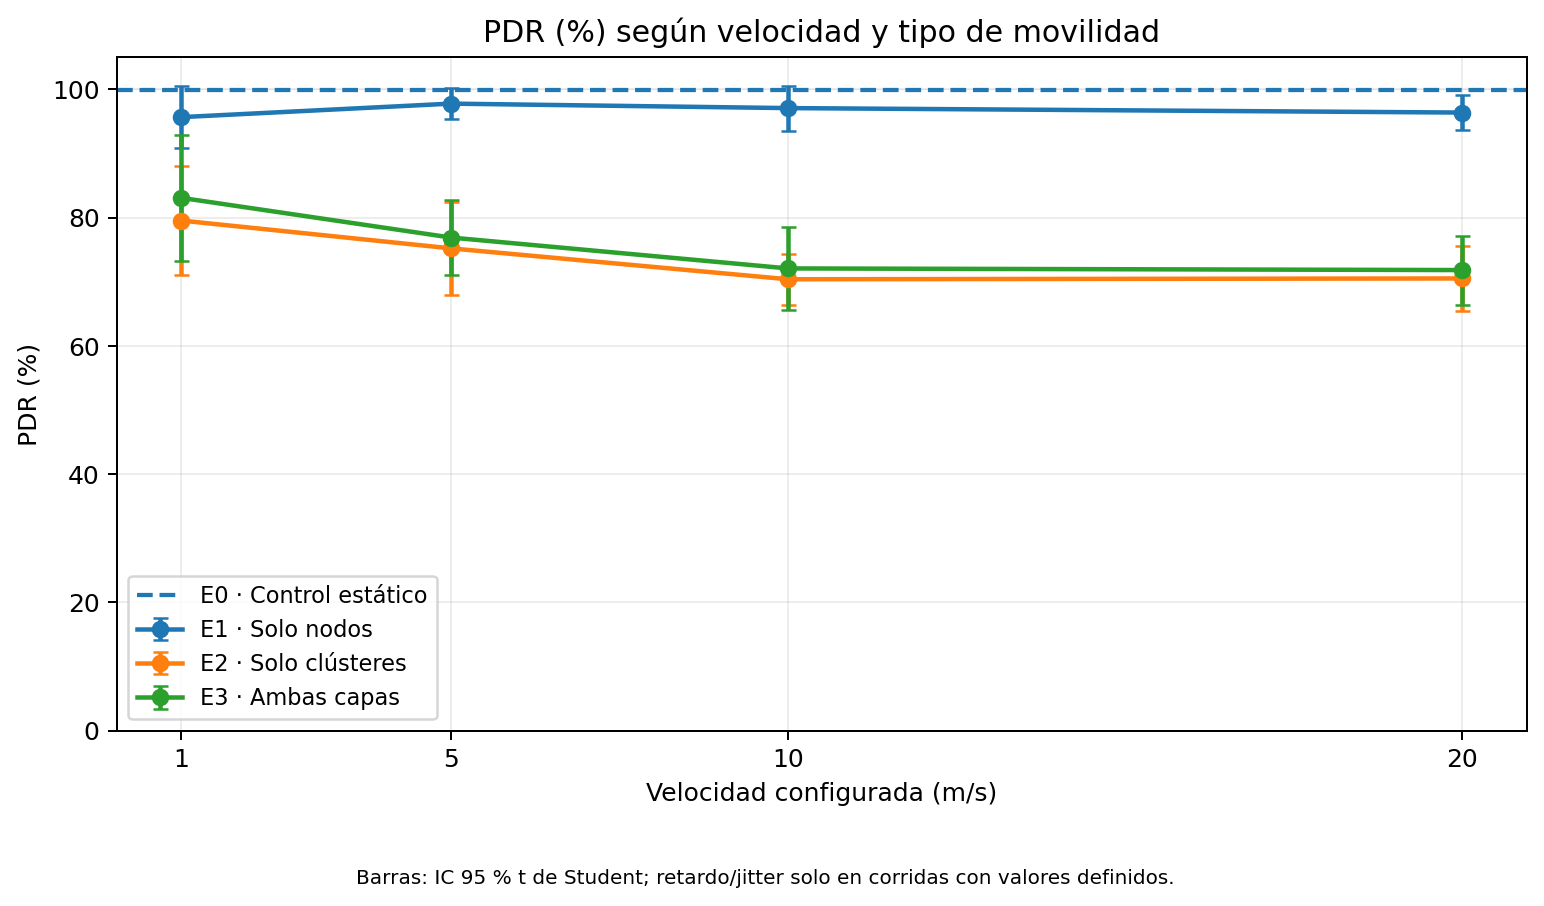
\includegraphics[width=0.75\textwidth]{resultados/figuras/01_pdr_vs_velocidad.png}
\caption{Ejemplo de gráfica generada por \texttt{graficar.py}: PDR contra velocidad
para cada escenario.}
\label{fig:manual-pdr}
\end{figure}

En las gráficas (figura~\ref{fig:manual-pdr}), cada punto es la media de las réplicas
de una configuración y las barras son su intervalo de confianza del 95\,\%. Cuando los
intervalos de dos escenarios no se traslapan, la diferencia entre ellos es clara; cuando
se traslapan, hay que mirar la prueba estadística.

En \texttt{tabla\_\allowbreak{}estadistica.csv}, las columnas que terminan en \texttt{\_\allowbreak{}media},
\texttt{\_\allowbreak{}ic95\_\allowbreak{}inf} y \texttt{\_\allowbreak{}ic95\_\allowbreak{}sup} son la media y los límites del intervalo de
cada métrica, y \texttt{corridas\_\allowbreak{}sin\_\allowbreak{}rx} cuenta las réplicas en las que no llegó
ningún paquete. En esas réplicas el retardo y el \emph{jitter} no se pueden calcular, así
que quedan vacíos en lugar de valer cero.

{\sloppy
En \texttt{comparacion\_\allowbreak{}E2\_\allowbreak{}vs\_\allowbreak{}E1.csv}, cada fila es una velocidad y una métrica. Las
columnas más importantes son \texttt{diferencia\_\allowbreak{}E2\_\allowbreak{}menos\_\allowbreak{}E1}, \texttt{p\_\allowbreak{}unilateral}
y \texttt{rechaza\_\allowbreak{}H0\_\allowbreak{}alpha\_\allowbreak{}0\_\allowbreak{}05}: si esta última vale \texttt{True}, la diferencia
va en la dirección de la hipótesis y es significativa con $\alpha = 0.05$. Según la
regla de decisión del informe (sección «Método de análisis estadístico»), la hipótesis
principal se respalda si eso ocurre en al menos tres de las cuatro velocidades.\par}

\subsection{Visualizar una simulación con NetAnim}

{\sloppy
Con \texttt{-{}-netanim=true}, el programa guarda en la carpeta de salida el archivo
\texttt{netanim\_\allowbreak{}<escenario>\_\allowbreak{}cs<clusterSpeed>\_\allowbreak{}ns<nodeSpeed>\_\allowbreak{}run<RngRun>.xml}. Al
abrirlo con NetAnim, que viene con ns-allinone, se ve el movimiento de los nodos: los CH
en rojo y los miembros en azul.\par}

\subsection{Problemas frecuentes}

\begin{center}
\small
\begin{tabular}{p{5.2cm}p{7.4cm}}
\toprule
\textbf{Mensaje o síntoma} & \textbf{Qué hacer} \\
\midrule
\texttt{No está ./ns3 en ...} o \texttt{No existe el directorio de ns-3} & Indicar la carpeta correcta con \texttt{-{}-ns3} o con la variable \texttt{NS3\_\allowbreak{}DIR}. \\
\texttt{OMITIDO (XML existente)} & Es normal al retomar un experimento. Para repetir esas simulaciones, agregar \texttt{-{}-forzar}. \\
\texttt{ERROR de simulación} & Revisar el archivo de esa simulación en \texttt{resultados/logs/}; el script muestra sus últimas líneas. \\
\texttt{./ns3} no arranca con el Python del sistema & Indicar otro intérprete con la variable \texttt{NS3\_\allowbreak{}PYTHON}. \\
Todo es muy lento en WSL & Mover ns-3 y el repositorio al disco de Linux (\texttt{\textasciitilde}) en vez de \texttt{/mnt/c/...}. \\
\bottomrule
\end{tabular}
\end{center}
.
% Usa los paquetes graphicx y booktabs, y las rutas son relativas a la
% raíz del repositorio.
% =====================================================================
\section{Manual de usuario}
\label{sec:manual-usuario}

Este manual explica, paso a paso, cómo correr una simulación, cómo correr todos los
escenarios del experimento, cómo generar las tablas y las gráficas y cómo leer los
resultados. La instalación de ns-3 y la estructura del código están en el manual
técnico.

\subsection{Antes de empezar}

Se necesita:

\begin{itemize}
    \item Ubuntu 22.04, nativo o en WSL2 sobre Windows.
    \item ns-3.43 compilado con los módulos \texttt{wifi}, \texttt{aodv},
    \texttt{mobility}, \texttt{internet}, \texttt{applications}, \texttt{flow-monitor}
    y \texttt{netanim} (ver el manual técnico).
    \item Python 3.10 o superior. Los scripts que corren y procesan las simulaciones solo
    usan la librería estándar; el de las gráficas necesita además \texttt{pandas},
    \texttt{matplotlib}, \texttt{scipy} y \texttt{numpy}.
    \item El repositorio del grupo, descargado en el disco de Linux (por ejemplo, en la
    carpeta personal \texttt{\textasciitilde}). En WSL no conviene trabajar en
    \texttt{/mnt/c/...}, porque compilar sobre el disco de Windows es mucho más lento.
\end{itemize}

\begin{verbatim}
cd ~
git clone https://github.com/10scar/tallerme01
cd tallerme01
python3 -m pip install pandas matplotlib scipy numpy
\end{verbatim}

En los ejemplos se supone que ns-3 está en \texttt{\textasciitilde/ns-allinone-3.43/ns-3.43}
y el repositorio en \texttt{\textasciitilde/tallerme01}; si están en otro lugar, basta
con cambiar esas rutas.

\subsection{Paso 1: correr una simulación}

El programa está en \texttt{simulacion/manet-jerarquica.cc}. ns-3 compila los programas
de su carpeta \texttt{scratch/}, así que primero se copia allí y luego se ejecuta desde
la carpeta de ns-3:

\begin{verbatim}
cp ~/tallerme01/simulacion/manet-jerarquica.cc ~/ns-allinone-3.43/ns-3.43/scratch/
cd ~/ns-allinone-3.43/ns-3.43
./ns3 run "scratch/manet-jerarquica --scenario=E3 --clusterSpeed=5 \
    --nodeSpeed=5 --simTime=200 --RngRun=1 \
    --outDir=$HOME/tallerme01/resultados/raw"
\end{verbatim}

La primera vez, \texttt{./ns3 run} compila el programa antes de ejecutarlo. Los
parámetros se pasan como \texttt{-{}-nombre=valor}; la tabla~\ref{tab:manual-parametros}
resume los que se usan. El nombre del escenario es solo una etiqueta: lo que define qué
se mueve son las velocidades. Por eso cada escenario se corre con esta combinación,
donde $v$ es la velocidad en m/s:

\begin{center}
\small
\begin{tabular}{lll}
\toprule
\textbf{Escenario} & \texttt{-{}-clusterSpeed} & \texttt{-{}-nodeSpeed} \\
\midrule
E0 (nada se mueve) & 0 & 0 \\
E1 (solo los nodos) & 0 & $v$ \\
E2 (solo los clústeres) & $v$ & 0 \\
E3 (ambos) & $v$ & $v$ \\
\bottomrule
\end{tabular}
\end{center}

\begin{table}[h]
\centering
\small
\begin{tabular}{p{3.4cm}p{1.6cm}p{7.4cm}}
\toprule
\textbf{Parámetro} & \textbf{Por defecto} & \textbf{Qué hace} \\
\midrule
\texttt{-{}-scenario} & \texttt{E3} & Etiqueta del escenario (E0 a E3); aparece en el nombre del archivo de salida. \\
\texttt{-{}-clusterSpeed} & 5 & Velocidad de los clústeres (m/s); 0 los deja quietos. \\
\texttt{-{}-nodeSpeed} & 5 & Velocidad de los nodos dentro de su clúster (m/s); 0 los deja quietos. \\
\texttt{-{}-superSpeed} & 0 & Velocidad de los superclústeres (m/s); en los experimentos es 0. \\
\texttt{-{}-simTime} & 200 & Duración de la simulación (s). \\
\texttt{-{}-RngRun} & 1 & Número de réplica: cada valor da una corrida independiente. \\
\texttt{-{}-outDir} & \texttt{resultados/\allowbreak{}raw} & Carpeta donde se guarda el XML de FlowMonitor; se crea si no existe. \\
\texttt{-{}-netanim} & \texttt{false} & Genera además una traza para NetAnim. \\
\texttt{-{}-verificar} & \texttt{false} & Corre la prueba de conectividad (paso 2). \\
\texttt{-{}-rangoCluster} & 60 & Alcance de radio dentro de cada clúster (m). \\
\texttt{-{}-rangoBackbone} & 250 & Alcance de radio entre CH (m). \\
\texttt{-{}-regionCluster} & 150 & Semiancho de la región en que se mueve cada clúster (m). \\
\texttt{-{}-regionNodo} & 40 & Semiancho de la región en que se mueve cada nodo (m). \\
\texttt{-{}-trazaPosiciones} & 0 & Imprime las posiciones cada tantos segundos (0 = no). \\
\bottomrule
\end{tabular}
\caption{Parámetros del programa \texttt{manet-jerarquica}.}
\label{tab:manual-parametros}
\end{table}

{\sloppy
Al empezar, el programa imprime la configuración de la red (clústeres, nodos, CH,
direcciones y posiciones iniciales). Al terminar, guarda el archivo
\texttt{<escenario>\_\allowbreak{}cs<clusterSpeed>\_\allowbreak{}ns<nodeSpeed>\_\allowbreak{}run<RngRun>.xml} en la carpeta de
salida e imprime un resumen con este formato:\par}

\begin{verbatim}
=== Métricas (FlowMonitor) ===
 Archivo:    <ruta del XML>
 Paquetes:   <recibidos>/<enviados> recibidos
 PDR:        <porcentaje> %
 Throughput: <valor> kbit/s
 Retardo:    <valor> s
 Jitter:     <valor> s
\end{verbatim}

Este resumen sirve para comprobar rápido que la corrida funcionó, pero suma todos los
flujos, incluidos los mensajes de control de AODV. Las cifras del informe salen de los
scripts del paso 4, que cuentan solo los flujos de datos, así que no coinciden con las de
la consola.

\subsection{Paso 2 (opcional): comprobar que todo funciona}

Para verificar que la red jerárquica está conectada, se corre el programa con
\texttt{-{}-verificar=true}. Envía paquetes de prueba entre clústeres y termina con el
mensaje \texttt{RESULTADO: la red jerárquica está conectada.} Si aparece
\texttt{RESULTADO: hay pares sin conectividad}, hay que revisar la geometría o los
alcances.

Para comprobar que la movilidad hace lo que dice el diseño, se corre desde la carpeta
del repositorio:

\begin{verbatim}
cd ~/tallerme01
python3 scripts/validar_movilidad.py --ns3 ~/ns-allinone-3.43/ns-3.43
\end{verbatim}

El script copia la versión actual del programa a \texttt{scratch/}, lo compila, corre
simulaciones cortas y revisa siete reglas: que en E0 nada se mueva, que en E1 solo se
muevan los miembros, que en E2 cada clúster viaje junto, que nadie salga de su región,
que las velocidades sean las pedidas, que la misma semilla dé el mismo resultado y que
haya ocho flujos de datos. Termina con código 0 si todas las pruebas pasan.

\subsection{Paso 3: correr todos los escenarios}

El script \texttt{scripts/correr\_\allowbreak{}escenarios.sh} corre el experimento completo: E0 una
vez y E1, E2 y E3 a 1, 5, 10 y 20\,m/s, con 10 réplicas cada uno, es decir, 130
simulaciones. Antes de empezar copia el programa a \texttt{scratch/}. Conviene probarlo
en este orden:

\begin{verbatim}
cd ~/tallerme01
bash scripts/correr_escenarios.sh --ns3 ~/ns-allinone-3.43/ns-3.43 --dry-run
bash scripts/correr_escenarios.sh --ns3 ~/ns-allinone-3.43/ns-3.43 --piloto
bash scripts/correr_escenarios.sh --ns3 ~/ns-allinone-3.43/ns-3.43
\end{verbatim}

La primera línea solo muestra los 130 comandos sin ejecutarlos; la segunda corre cuatro
simulaciones de prueba (E0, y E1, E2 y E3 a 5\,m/s), y la tercera corre todo. Mientras
avanza, el script muestra una línea por simulación, por ejemplo
\texttt{[012/130] Ejecutando E1\_\allowbreak{}cs0\_\allowbreak{}ns1\_\allowbreak{}run2 ... OK}. Las opciones son:

\begin{center}
\small
\begin{tabular}{p{3.6cm}p{9cm}}
\toprule
\textbf{Opción} & \textbf{Qué hace} \\
\midrule
\texttt{-{}-ns3 RUTA} & Carpeta de ns-3 que contiene \texttt{./ns3}. También se puede dar con la variable \texttt{NS3\_\allowbreak{}DIR}. \\
\texttt{-{}-repeticiones N} & Réplicas por configuración (por defecto, 10). \\
\texttt{-{}-piloto} & Corre solo cuatro simulaciones de prueba. \\
\texttt{-{}-dry-run} & Muestra los comandos sin ejecutar nada. \\
\texttt{-{}-forzar} & Repite las simulaciones aunque ya exista su XML. \\
\texttt{-{}-sin-copiar} & No copia el programa a \texttt{scratch/}. \\
\texttt{-{}-ayuda} & Muestra la ayuda. \\
\bottomrule
\end{tabular}
\end{center}

Los XML quedan en \texttt{resultados/raw/} y la salida de cada simulación en
\texttt{resultados/logs/}. Si el experimento se interrumpe, basta con volver a correr el
mismo comando: las simulaciones que ya tienen su XML se omiten
(\texttt{OMITIDO (XML existente)}).

\subsection{Paso 4: procesar los resultados}

\begin{verbatim}
python3 scripts/parse_flowmon.py
\end{verbatim}

Este script lee todos los XML de \texttt{resultados/raw/} y escribe
\texttt{resultados/resumen.csv}, con una fila por simulación. Solo cuenta los ocho flujos
de datos (puertos UDP 5000 a 5007) y deja por fuera el tráfico de control de AODV
(puerto 654). Sus opciones son \texttt{-{}-raw} (carpeta de los XML), \texttt{-{}-salida}
(archivo CSV), \texttt{-{}-sim-time} (duración de cada simulación, 200\,s por defecto),
\texttt{-{}-completo} (exige que estén las 13 configuraciones con todas sus réplicas) y
\texttt{-{}-repeticiones}.

Las columnas principales de \texttt{resumen.csv} son el escenario, las velocidades, la
réplica (\texttt{run}), los paquetes enviados y recibidos (\texttt{tx\_\allowbreak{}packets},
\texttt{rx\_\allowbreak{}packets}) y las cuatro métricas: \texttt{pdr\_\allowbreak{}pct} (\%),
\texttt{retardo\_\allowbreak{}ms}, \texttt{throughput\_\allowbreak{}kbps} y \texttt{jitter\_\allowbreak{}ms}.

\subsection{Paso 5: generar las gráficas y las pruebas estadísticas}

\begin{verbatim}
python3 scripts/graficar.py
\end{verbatim}

A partir de \texttt{resumen.csv}, el script genera:

\begin{itemize}
    \item \texttt{resultados/figuras/}: cinco gráficas, una por métrica contra la
    velocidad (\texttt{01\_\allowbreak{}pdr}, \texttt{02\_\allowbreak{}retardo}, \texttt{03\_\allowbreak{}throughput},
    \texttt{04\_\allowbreak{}jitter}) y una con las corridas en las que no llegó ningún paquete
    (\texttt{05\_\allowbreak{}corridas\_\allowbreak{}sin\_\allowbreak{}recepcion}).
    \item \texttt{resultados/tabla\_\allowbreak{}estadistica.csv}: media, desviación estándar e
    intervalo de confianza del 95\,\% de cada métrica, por escenario y velocidad.
    \item \texttt{resultados/comparacion\_\allowbreak{}E2\_\allowbreak{}vs\_\allowbreak{}E1.csv}: la prueba $t$ de Welch
    unilateral entre E2 y E1 para cada velocidad.
    \item \texttt{resultados/RESULTADOS.md}: un resumen con las figuras y la tabla
    principal.
\end{itemize}

Sus opciones \texttt{-{}-csv}, \texttt{-{}-figuras} y \texttt{-{}-resultados} permiten cambiar
el archivo de entrada y las carpetas de salida.

\subsection{Paso 6: interpretar los resultados}

\begin{figure}[h]
\centering
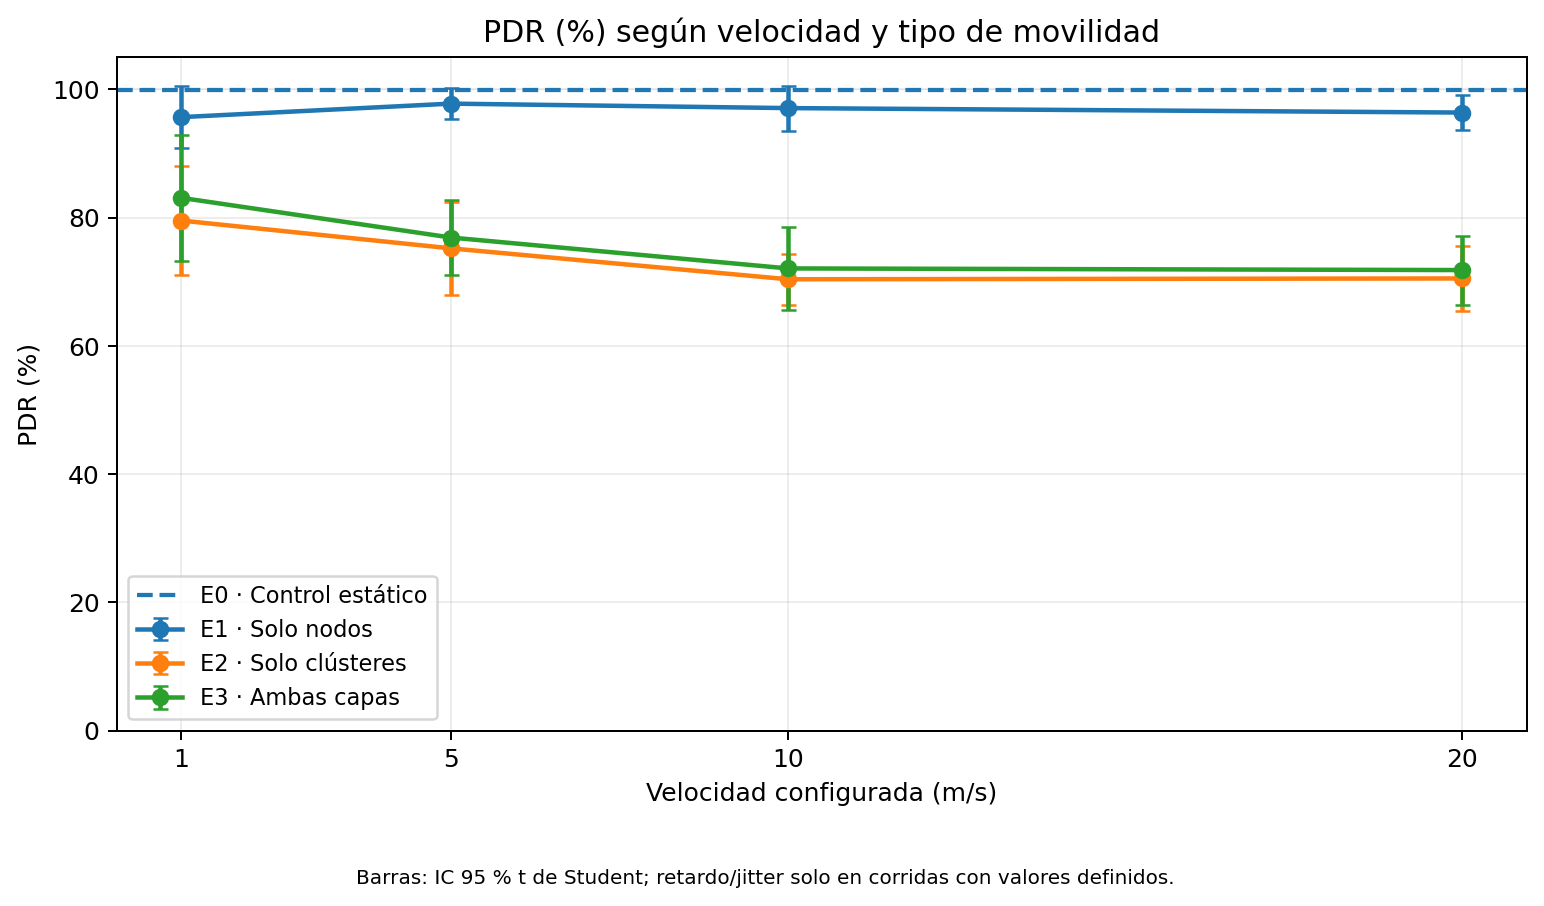
\includegraphics[width=0.75\textwidth]{resultados/figuras/01_pdr_vs_velocidad.png}
\caption{Ejemplo de gráfica generada por \texttt{graficar.py}: PDR contra velocidad
para cada escenario.}
\label{fig:manual-pdr}
\end{figure}

En las gráficas (figura~\ref{fig:manual-pdr}), cada punto es la media de las réplicas
de una configuración y las barras son su intervalo de confianza del 95\,\%. Cuando los
intervalos de dos escenarios no se traslapan, la diferencia entre ellos es clara; cuando
se traslapan, hay que mirar la prueba estadística.

En \texttt{tabla\_\allowbreak{}estadistica.csv}, las columnas que terminan en \texttt{\_\allowbreak{}media},
\texttt{\_\allowbreak{}ic95\_\allowbreak{}inf} y \texttt{\_\allowbreak{}ic95\_\allowbreak{}sup} son la media y los límites del intervalo de
cada métrica, y \texttt{corridas\_\allowbreak{}sin\_\allowbreak{}rx} cuenta las réplicas en las que no llegó
ningún paquete. En esas réplicas el retardo y el \emph{jitter} no se pueden calcular, así
que quedan vacíos en lugar de valer cero.

{\sloppy
En \texttt{comparacion\_\allowbreak{}E2\_\allowbreak{}vs\_\allowbreak{}E1.csv}, cada fila es una velocidad y una métrica. Las
columnas más importantes son \texttt{diferencia\_\allowbreak{}E2\_\allowbreak{}menos\_\allowbreak{}E1}, \texttt{p\_\allowbreak{}unilateral}
y \texttt{rechaza\_\allowbreak{}H0\_\allowbreak{}alpha\_\allowbreak{}0\_\allowbreak{}05}: si esta última vale \texttt{True}, la diferencia
va en la dirección de la hipótesis y es significativa con $\alpha = 0.05$. Según la
regla de decisión del informe (sección «Método de análisis estadístico»), la hipótesis
principal se respalda si eso ocurre en al menos tres de las cuatro velocidades.\par}

\subsection{Visualizar una simulación con NetAnim}

{\sloppy
Con \texttt{-{}-netanim=true}, el programa guarda en la carpeta de salida el archivo
\texttt{netanim\_\allowbreak{}<escenario>\_\allowbreak{}cs<clusterSpeed>\_\allowbreak{}ns<nodeSpeed>\_\allowbreak{}run<RngRun>.xml}. Al
abrirlo con NetAnim, que viene con ns-allinone, se ve el movimiento de los nodos: los CH
en rojo y los miembros en azul.\par}

\subsection{Problemas frecuentes}

\begin{center}
\small
\begin{tabular}{p{5.2cm}p{7.4cm}}
\toprule
\textbf{Mensaje o síntoma} & \textbf{Qué hacer} \\
\midrule
\texttt{No está ./ns3 en ...} o \texttt{No existe el directorio de ns-3} & Indicar la carpeta correcta con \texttt{-{}-ns3} o con la variable \texttt{NS3\_\allowbreak{}DIR}. \\
\texttt{OMITIDO (XML existente)} & Es normal al retomar un experimento. Para repetir esas simulaciones, agregar \texttt{-{}-forzar}. \\
\texttt{ERROR de simulación} & Revisar el archivo de esa simulación en \texttt{resultados/logs/}; el script muestra sus últimas líneas. \\
\texttt{./ns3} no arranca con el Python del sistema & Indicar otro intérprete con la variable \texttt{NS3\_\allowbreak{}PYTHON}. \\
Todo es muy lento en WSL & Mover ns-3 y el repositorio al disco de Linux (\texttt{\textasciitilde}) en vez de \texttt{/mnt/c/...}. \\
\bottomrule
\end{tabular}
\end{center}
.
% Usa los paquetes graphicx y booktabs, y las rutas son relativas a la
% raíz del repositorio.
% =====================================================================
\section{Manual de usuario}
\label{sec:manual-usuario}

Este manual explica, paso a paso, cómo correr una simulación, cómo correr todos los
escenarios del experimento, cómo generar las tablas y las gráficas y cómo leer los
resultados. La instalación de ns-3 y la estructura del código están en el manual
técnico.

\subsection{Antes de empezar}

Se necesita:

\begin{itemize}
    \item Ubuntu 22.04, nativo o en WSL2 sobre Windows.
    \item ns-3.43 compilado con los módulos \texttt{wifi}, \texttt{aodv},
    \texttt{mobility}, \texttt{internet}, \texttt{applications}, \texttt{flow-monitor}
    y \texttt{netanim} (ver el manual técnico).
    \item Python 3.10 o superior. Los scripts que corren y procesan las simulaciones solo
    usan la librería estándar; el de las gráficas necesita además \texttt{pandas},
    \texttt{matplotlib}, \texttt{scipy} y \texttt{numpy}.
    \item El repositorio del grupo, descargado en el disco de Linux (por ejemplo, en la
    carpeta personal \texttt{\textasciitilde}). En WSL no conviene trabajar en
    \texttt{/mnt/c/...}, porque compilar sobre el disco de Windows es mucho más lento.
\end{itemize}

\begin{verbatim}
cd ~
git clone https://github.com/10scar/tallerme01
cd tallerme01
python3 -m pip install pandas matplotlib scipy numpy
\end{verbatim}

En los ejemplos se supone que ns-3 está en \texttt{\textasciitilde/ns-allinone-3.43/ns-3.43}
y el repositorio en \texttt{\textasciitilde/tallerme01}; si están en otro lugar, basta
con cambiar esas rutas.

\subsection{Paso 1: correr una simulación}

El programa está en \texttt{simulacion/manet-jerarquica.cc}. ns-3 compila los programas
de su carpeta \texttt{scratch/}, así que primero se copia allí y luego se ejecuta desde
la carpeta de ns-3:

\begin{verbatim}
cp ~/tallerme01/simulacion/manet-jerarquica.cc ~/ns-allinone-3.43/ns-3.43/scratch/
cd ~/ns-allinone-3.43/ns-3.43
./ns3 run "scratch/manet-jerarquica --scenario=E3 --clusterSpeed=5 \
    --nodeSpeed=5 --simTime=200 --RngRun=1 \
    --outDir=$HOME/tallerme01/resultados/raw"
\end{verbatim}

La primera vez, \texttt{./ns3 run} compila el programa antes de ejecutarlo. Los
parámetros se pasan como \texttt{-{}-nombre=valor}; la tabla~\ref{tab:manual-parametros}
resume los que se usan. El nombre del escenario es solo una etiqueta: lo que define qué
se mueve son las velocidades. Por eso cada escenario se corre con esta combinación,
donde $v$ es la velocidad en m/s:

\begin{center}
\small
\begin{tabular}{lll}
\toprule
\textbf{Escenario} & \texttt{-{}-clusterSpeed} & \texttt{-{}-nodeSpeed} \\
\midrule
E0 (nada se mueve) & 0 & 0 \\
E1 (solo los nodos) & 0 & $v$ \\
E2 (solo los clústeres) & $v$ & 0 \\
E3 (ambos) & $v$ & $v$ \\
\bottomrule
\end{tabular}
\end{center}

\begin{table}[h]
\centering
\small
\begin{tabular}{p{3.4cm}p{1.6cm}p{7.4cm}}
\toprule
\textbf{Parámetro} & \textbf{Por defecto} & \textbf{Qué hace} \\
\midrule
\texttt{-{}-scenario} & \texttt{E3} & Etiqueta del escenario (E0 a E3); aparece en el nombre del archivo de salida. \\
\texttt{-{}-clusterSpeed} & 5 & Velocidad de los clústeres (m/s); 0 los deja quietos. \\
\texttt{-{}-nodeSpeed} & 5 & Velocidad de los nodos dentro de su clúster (m/s); 0 los deja quietos. \\
\texttt{-{}-superSpeed} & 0 & Velocidad de los superclústeres (m/s); en los experimentos es 0. \\
\texttt{-{}-simTime} & 200 & Duración de la simulación (s). \\
\texttt{-{}-RngRun} & 1 & Número de réplica: cada valor da una corrida independiente. \\
\texttt{-{}-outDir} & \texttt{resultados/\allowbreak{}raw} & Carpeta donde se guarda el XML de FlowMonitor; se crea si no existe. \\
\texttt{-{}-netanim} & \texttt{false} & Genera además una traza para NetAnim. \\
\texttt{-{}-verificar} & \texttt{false} & Corre la prueba de conectividad (paso 2). \\
\texttt{-{}-rangoCluster} & 60 & Alcance de radio dentro de cada clúster (m). \\
\texttt{-{}-rangoBackbone} & 250 & Alcance de radio entre CH (m). \\
\texttt{-{}-regionCluster} & 150 & Semiancho de la región en que se mueve cada clúster (m). \\
\texttt{-{}-regionNodo} & 40 & Semiancho de la región en que se mueve cada nodo (m). \\
\texttt{-{}-trazaPosiciones} & 0 & Imprime las posiciones cada tantos segundos (0 = no). \\
\bottomrule
\end{tabular}
\caption{Parámetros del programa \texttt{manet-jerarquica}.}
\label{tab:manual-parametros}
\end{table}

{\sloppy
Al empezar, el programa imprime la configuración de la red (clústeres, nodos, CH,
direcciones y posiciones iniciales). Al terminar, guarda el archivo
\texttt{<escenario>\_\allowbreak{}cs<clusterSpeed>\_\allowbreak{}ns<nodeSpeed>\_\allowbreak{}run<RngRun>.xml} en la carpeta de
salida e imprime un resumen con este formato:\par}

\begin{verbatim}
=== Métricas (FlowMonitor) ===
 Archivo:    <ruta del XML>
 Paquetes:   <recibidos>/<enviados> recibidos
 PDR:        <porcentaje> %
 Throughput: <valor> kbit/s
 Retardo:    <valor> s
 Jitter:     <valor> s
\end{verbatim}

Este resumen sirve para comprobar rápido que la corrida funcionó, pero suma todos los
flujos, incluidos los mensajes de control de AODV. Las cifras del informe salen de los
scripts del paso 4, que cuentan solo los flujos de datos, así que no coinciden con las de
la consola.

\subsection{Paso 2 (opcional): comprobar que todo funciona}

Para verificar que la red jerárquica está conectada, se corre el programa con
\texttt{-{}-verificar=true}. Envía paquetes de prueba entre clústeres y termina con el
mensaje \texttt{RESULTADO: la red jerárquica está conectada.} Si aparece
\texttt{RESULTADO: hay pares sin conectividad}, hay que revisar la geometría o los
alcances.

Para comprobar que la movilidad hace lo que dice el diseño, se corre desde la carpeta
del repositorio:

\begin{verbatim}
cd ~/tallerme01
python3 scripts/validar_movilidad.py --ns3 ~/ns-allinone-3.43/ns-3.43
\end{verbatim}

El script copia la versión actual del programa a \texttt{scratch/}, lo compila, corre
simulaciones cortas y revisa siete reglas: que en E0 nada se mueva, que en E1 solo se
muevan los miembros, que en E2 cada clúster viaje junto, que nadie salga de su región,
que las velocidades sean las pedidas, que la misma semilla dé el mismo resultado y que
haya ocho flujos de datos. Termina con código 0 si todas las pruebas pasan.

\subsection{Paso 3: correr todos los escenarios}

El script \texttt{scripts/correr\_\allowbreak{}escenarios.sh} corre el experimento completo: E0 una
vez y E1, E2 y E3 a 1, 5, 10 y 20\,m/s, con 10 réplicas cada uno, es decir, 130
simulaciones. Antes de empezar copia el programa a \texttt{scratch/}. Conviene probarlo
en este orden:

\begin{verbatim}
cd ~/tallerme01
bash scripts/correr_escenarios.sh --ns3 ~/ns-allinone-3.43/ns-3.43 --dry-run
bash scripts/correr_escenarios.sh --ns3 ~/ns-allinone-3.43/ns-3.43 --piloto
bash scripts/correr_escenarios.sh --ns3 ~/ns-allinone-3.43/ns-3.43
\end{verbatim}

La primera línea solo muestra los 130 comandos sin ejecutarlos; la segunda corre cuatro
simulaciones de prueba (E0, y E1, E2 y E3 a 5\,m/s), y la tercera corre todo. Mientras
avanza, el script muestra una línea por simulación, por ejemplo
\texttt{[012/130] Ejecutando E1\_\allowbreak{}cs0\_\allowbreak{}ns1\_\allowbreak{}run2 ... OK}. Las opciones son:

\begin{center}
\small
\begin{tabular}{p{3.6cm}p{9cm}}
\toprule
\textbf{Opción} & \textbf{Qué hace} \\
\midrule
\texttt{-{}-ns3 RUTA} & Carpeta de ns-3 que contiene \texttt{./ns3}. También se puede dar con la variable \texttt{NS3\_\allowbreak{}DIR}. \\
\texttt{-{}-repeticiones N} & Réplicas por configuración (por defecto, 10). \\
\texttt{-{}-piloto} & Corre solo cuatro simulaciones de prueba. \\
\texttt{-{}-dry-run} & Muestra los comandos sin ejecutar nada. \\
\texttt{-{}-forzar} & Repite las simulaciones aunque ya exista su XML. \\
\texttt{-{}-sin-copiar} & No copia el programa a \texttt{scratch/}. \\
\texttt{-{}-ayuda} & Muestra la ayuda. \\
\bottomrule
\end{tabular}
\end{center}

Los XML quedan en \texttt{resultados/raw/} y la salida de cada simulación en
\texttt{resultados/logs/}. Si el experimento se interrumpe, basta con volver a correr el
mismo comando: las simulaciones que ya tienen su XML se omiten
(\texttt{OMITIDO (XML existente)}).

\subsection{Paso 4: procesar los resultados}

\begin{verbatim}
python3 scripts/parse_flowmon.py
\end{verbatim}

Este script lee todos los XML de \texttt{resultados/raw/} y escribe
\texttt{resultados/resumen.csv}, con una fila por simulación. Solo cuenta los ocho flujos
de datos (puertos UDP 5000 a 5007) y deja por fuera el tráfico de control de AODV
(puerto 654). Sus opciones son \texttt{-{}-raw} (carpeta de los XML), \texttt{-{}-salida}
(archivo CSV), \texttt{-{}-sim-time} (duración de cada simulación, 200\,s por defecto),
\texttt{-{}-completo} (exige que estén las 13 configuraciones con todas sus réplicas) y
\texttt{-{}-repeticiones}.

Las columnas principales de \texttt{resumen.csv} son el escenario, las velocidades, la
réplica (\texttt{run}), los paquetes enviados y recibidos (\texttt{tx\_\allowbreak{}packets},
\texttt{rx\_\allowbreak{}packets}) y las cuatro métricas: \texttt{pdr\_\allowbreak{}pct} (\%),
\texttt{retardo\_\allowbreak{}ms}, \texttt{throughput\_\allowbreak{}kbps} y \texttt{jitter\_\allowbreak{}ms}.

\subsection{Paso 5: generar las gráficas y las pruebas estadísticas}

\begin{verbatim}
python3 scripts/graficar.py
\end{verbatim}

A partir de \texttt{resumen.csv}, el script genera:

\begin{itemize}
    \item \texttt{resultados/figuras/}: cinco gráficas, una por métrica contra la
    velocidad (\texttt{01\_\allowbreak{}pdr}, \texttt{02\_\allowbreak{}retardo}, \texttt{03\_\allowbreak{}throughput},
    \texttt{04\_\allowbreak{}jitter}) y una con las corridas en las que no llegó ningún paquete
    (\texttt{05\_\allowbreak{}corridas\_\allowbreak{}sin\_\allowbreak{}recepcion}).
    \item \texttt{resultados/tabla\_\allowbreak{}estadistica.csv}: media, desviación estándar e
    intervalo de confianza del 95\,\% de cada métrica, por escenario y velocidad.
    \item \texttt{resultados/comparacion\_\allowbreak{}E2\_\allowbreak{}vs\_\allowbreak{}E1.csv}: la prueba $t$ de Welch
    unilateral entre E2 y E1 para cada velocidad.
    \item \texttt{resultados/RESULTADOS.md}: un resumen con las figuras y la tabla
    principal.
\end{itemize}

Sus opciones \texttt{-{}-csv}, \texttt{-{}-figuras} y \texttt{-{}-resultados} permiten cambiar
el archivo de entrada y las carpetas de salida.

\subsection{Paso 6: interpretar los resultados}

\begin{figure}[h]
\centering
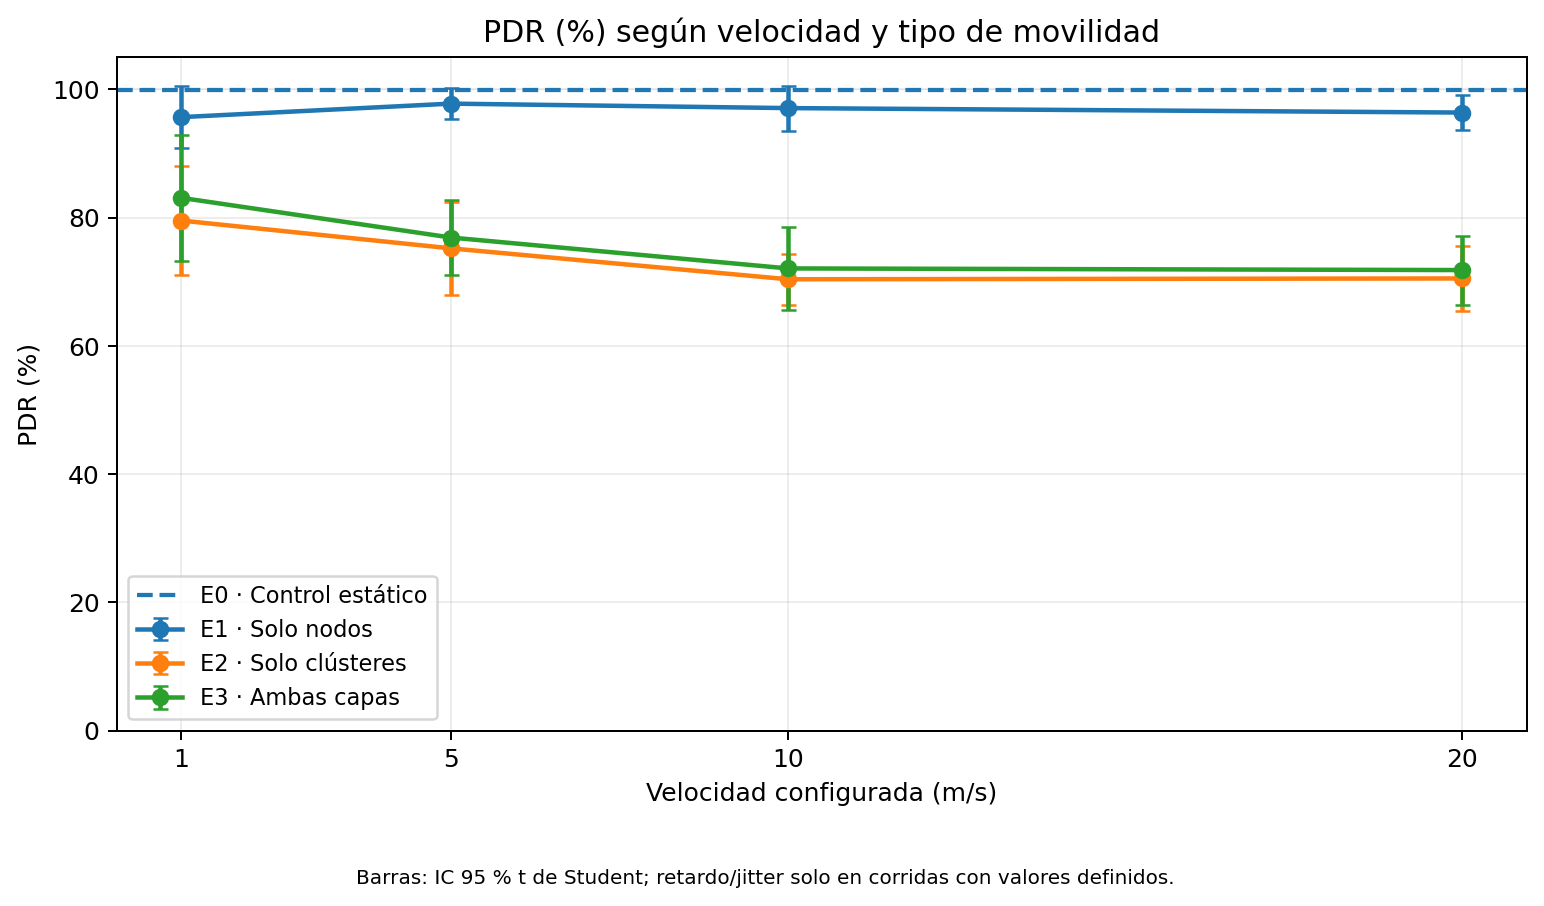
\includegraphics[width=0.75\textwidth]{resultados/figuras/01_pdr_vs_velocidad.png}
\caption{Ejemplo de gráfica generada por \texttt{graficar.py}: PDR contra velocidad
para cada escenario.}
\label{fig:manual-pdr}
\end{figure}

En las gráficas (figura~\ref{fig:manual-pdr}), cada punto es la media de las réplicas
de una configuración y las barras son su intervalo de confianza del 95\,\%. Cuando los
intervalos de dos escenarios no se traslapan, la diferencia entre ellos es clara; cuando
se traslapan, hay que mirar la prueba estadística.

En \texttt{tabla\_\allowbreak{}estadistica.csv}, las columnas que terminan en \texttt{\_\allowbreak{}media},
\texttt{\_\allowbreak{}ic95\_\allowbreak{}inf} y \texttt{\_\allowbreak{}ic95\_\allowbreak{}sup} son la media y los límites del intervalo de
cada métrica, y \texttt{corridas\_\allowbreak{}sin\_\allowbreak{}rx} cuenta las réplicas en las que no llegó
ningún paquete. En esas réplicas el retardo y el \emph{jitter} no se pueden calcular, así
que quedan vacíos en lugar de valer cero.

{\sloppy
En \texttt{comparacion\_\allowbreak{}E2\_\allowbreak{}vs\_\allowbreak{}E1.csv}, cada fila es una velocidad y una métrica. Las
columnas más importantes son \texttt{diferencia\_\allowbreak{}E2\_\allowbreak{}menos\_\allowbreak{}E1}, \texttt{p\_\allowbreak{}unilateral}
y \texttt{rechaza\_\allowbreak{}H0\_\allowbreak{}alpha\_\allowbreak{}0\_\allowbreak{}05}: si esta última vale \texttt{True}, la diferencia
va en la dirección de la hipótesis y es significativa con $\alpha = 0.05$. Según la
regla de decisión del informe (sección «Método de análisis estadístico»), la hipótesis
principal se respalda si eso ocurre en al menos tres de las cuatro velocidades.\par}

\subsection{Visualizar una simulación con NetAnim}

{\sloppy
Con \texttt{-{}-netanim=true}, el programa guarda en la carpeta de salida el archivo
\texttt{netanim\_\allowbreak{}<escenario>\_\allowbreak{}cs<clusterSpeed>\_\allowbreak{}ns<nodeSpeed>\_\allowbreak{}run<RngRun>.xml}. Al
abrirlo con NetAnim, que viene con ns-allinone, se ve el movimiento de los nodos: los CH
en rojo y los miembros en azul.\par}

\subsection{Problemas frecuentes}

\begin{center}
\small
\begin{tabular}{p{5.2cm}p{7.4cm}}
\toprule
\textbf{Mensaje o síntoma} & \textbf{Qué hacer} \\
\midrule
\texttt{No está ./ns3 en ...} o \texttt{No existe el directorio de ns-3} & Indicar la carpeta correcta con \texttt{-{}-ns3} o con la variable \texttt{NS3\_\allowbreak{}DIR}. \\
\texttt{OMITIDO (XML existente)} & Es normal al retomar un experimento. Para repetir esas simulaciones, agregar \texttt{-{}-forzar}. \\
\texttt{ERROR de simulación} & Revisar el archivo de esa simulación en \texttt{resultados/logs/}; el script muestra sus últimas líneas. \\
\texttt{./ns3} no arranca con el Python del sistema & Indicar otro intérprete con la variable \texttt{NS3\_\allowbreak{}PYTHON}. \\
Todo es muy lento en WSL & Mover ns-3 y el repositorio al disco de Linux (\texttt{\textasciitilde}) en vez de \texttt{/mnt/c/...}. \\
\bottomrule
\end{tabular}
\end{center}
.
% Usa los paquetes graphicx y booktabs, y las rutas son relativas a la
% raíz del repositorio.
% =====================================================================
\section{Manual de usuario}
\label{sec:manual-usuario}

Este manual explica, paso a paso, cómo correr una simulación, cómo correr todos los
escenarios del experimento, cómo generar las tablas y las gráficas y cómo leer los
resultados. La instalación de ns-3 y la estructura del código están en el manual
técnico.

\subsection{Antes de empezar}

Se necesita:

\begin{itemize}
    \item Ubuntu 22.04, nativo o en WSL2 sobre Windows.
    \item ns-3.43 compilado con los módulos \texttt{wifi}, \texttt{aodv},
    \texttt{mobility}, \texttt{internet}, \texttt{applications}, \texttt{flow-monitor}
    y \texttt{netanim} (ver el manual técnico).
    \item Python 3.10 o superior. Los scripts que corren y procesan las simulaciones solo
    usan la librería estándar; el de las gráficas necesita además \texttt{pandas},
    \texttt{matplotlib}, \texttt{scipy} y \texttt{numpy}.
    \item El repositorio del grupo, descargado en el disco de Linux (por ejemplo, en la
    carpeta personal \texttt{\textasciitilde}). En WSL no conviene trabajar en
    \texttt{/mnt/c/...}, porque compilar sobre el disco de Windows es mucho más lento.
\end{itemize}

\begin{verbatim}
cd ~
git clone https://github.com/10scar/tallerme01
cd tallerme01
python3 -m pip install pandas matplotlib scipy numpy
\end{verbatim}

En los ejemplos se supone que ns-3 está en \texttt{\textasciitilde/ns-allinone-3.43/ns-3.43}
y el repositorio en \texttt{\textasciitilde/tallerme01}; si están en otro lugar, basta
con cambiar esas rutas.

\subsection{Paso 1: correr una simulación}

El programa está en \texttt{simulacion/manet-jerarquica.cc}. ns-3 compila los programas
de su carpeta \texttt{scratch/}, así que primero se copia allí y luego se ejecuta desde
la carpeta de ns-3:

\begin{verbatim}
cp ~/tallerme01/simulacion/manet-jerarquica.cc ~/ns-allinone-3.43/ns-3.43/scratch/
cd ~/ns-allinone-3.43/ns-3.43
./ns3 run "scratch/manet-jerarquica --scenario=E3 --clusterSpeed=5 \
    --nodeSpeed=5 --simTime=200 --RngRun=1 \
    --outDir=$HOME/tallerme01/resultados/raw"
\end{verbatim}

La primera vez, \texttt{./ns3 run} compila el programa antes de ejecutarlo. Los
parámetros se pasan como \texttt{-{}-nombre=valor}; la tabla~\ref{tab:manual-parametros}
resume los que se usan. El nombre del escenario es solo una etiqueta: lo que define qué
se mueve son las velocidades. Por eso cada escenario se corre con esta combinación,
donde $v$ es la velocidad en m/s:

\begin{center}
\small
\begin{tabular}{lll}
\toprule
\textbf{Escenario} & \texttt{-{}-clusterSpeed} & \texttt{-{}-nodeSpeed} \\
\midrule
E0 (nada se mueve) & 0 & 0 \\
E1 (solo los nodos) & 0 & $v$ \\
E2 (solo los clústeres) & $v$ & 0 \\
E3 (ambos) & $v$ & $v$ \\
\bottomrule
\end{tabular}
\end{center}

\begin{table}[h]
\centering
\small
\begin{tabular}{p{3.4cm}p{1.6cm}p{7.4cm}}
\toprule
\textbf{Parámetro} & \textbf{Por defecto} & \textbf{Qué hace} \\
\midrule
\texttt{-{}-scenario} & \texttt{E3} & Etiqueta del escenario (E0 a E3); aparece en el nombre del archivo de salida. \\
\texttt{-{}-clusterSpeed} & 5 & Velocidad de los clústeres (m/s); 0 los deja quietos. \\
\texttt{-{}-nodeSpeed} & 5 & Velocidad de los nodos dentro de su clúster (m/s); 0 los deja quietos. \\
\texttt{-{}-superSpeed} & 0 & Velocidad de los superclústeres (m/s); en los experimentos es 0. \\
\texttt{-{}-simTime} & 200 & Duración de la simulación (s). \\
\texttt{-{}-RngRun} & 1 & Número de réplica: cada valor da una corrida independiente. \\
\texttt{-{}-outDir} & \texttt{resultados/\allowbreak{}raw} & Carpeta donde se guarda el XML de FlowMonitor; se crea si no existe. \\
\texttt{-{}-netanim} & \texttt{false} & Genera además una traza para NetAnim. \\
\texttt{-{}-verificar} & \texttt{false} & Corre la prueba de conectividad (paso 2). \\
\texttt{-{}-rangoCluster} & 60 & Alcance de radio dentro de cada clúster (m). \\
\texttt{-{}-rangoBackbone} & 250 & Alcance de radio entre CH (m). \\
\texttt{-{}-regionCluster} & 150 & Semiancho de la región en que se mueve cada clúster (m). \\
\texttt{-{}-regionNodo} & 40 & Semiancho de la región en que se mueve cada nodo (m). \\
\texttt{-{}-trazaPosiciones} & 0 & Imprime las posiciones cada tantos segundos (0 = no). \\
\bottomrule
\end{tabular}
\caption{Parámetros del programa \texttt{manet-jerarquica}.}
\label{tab:manual-parametros}
\end{table}

{\sloppy
Al empezar, el programa imprime la configuración de la red (clústeres, nodos, CH,
direcciones y posiciones iniciales). Al terminar, guarda el archivo
\texttt{<escenario>\_\allowbreak{}cs<clusterSpeed>\_\allowbreak{}ns<nodeSpeed>\_\allowbreak{}run<RngRun>.xml} en la carpeta de
salida e imprime un resumen con este formato:\par}

\begin{verbatim}
=== Métricas (FlowMonitor) ===
 Archivo:    <ruta del XML>
 Paquetes:   <recibidos>/<enviados> recibidos
 PDR:        <porcentaje> %
 Throughput: <valor> kbit/s
 Retardo:    <valor> s
 Jitter:     <valor> s
\end{verbatim}

Este resumen sirve para comprobar rápido que la corrida funcionó, pero suma todos los
flujos, incluidos los mensajes de control de AODV. Las cifras del informe salen de los
scripts del paso 4, que cuentan solo los flujos de datos, así que no coinciden con las de
la consola.

\subsection{Paso 2 (opcional): comprobar que todo funciona}

Para verificar que la red jerárquica está conectada, se corre el programa con
\texttt{-{}-verificar=true}. Envía paquetes de prueba entre clústeres y termina con el
mensaje \texttt{RESULTADO: la red jerárquica está conectada.} Si aparece
\texttt{RESULTADO: hay pares sin conectividad}, hay que revisar la geometría o los
alcances.

Para comprobar que la movilidad hace lo que dice el diseño, se corre desde la carpeta
del repositorio:

\begin{verbatim}
cd ~/tallerme01
python3 scripts/validar_movilidad.py --ns3 ~/ns-allinone-3.43/ns-3.43
\end{verbatim}

El script copia la versión actual del programa a \texttt{scratch/}, lo compila, corre
simulaciones cortas y revisa siete reglas: que en E0 nada se mueva, que en E1 solo se
muevan los miembros, que en E2 cada clúster viaje junto, que nadie salga de su región,
que las velocidades sean las pedidas, que la misma semilla dé el mismo resultado y que
haya ocho flujos de datos. Termina con código 0 si todas las pruebas pasan.

\subsection{Paso 3: correr todos los escenarios}

El script \texttt{scripts/correr\_\allowbreak{}escenarios.sh} corre el experimento completo: E0 una
vez y E1, E2 y E3 a 1, 5, 10 y 20\,m/s, con 10 réplicas cada uno, es decir, 130
simulaciones. Antes de empezar copia el programa a \texttt{scratch/}. Conviene probarlo
en este orden:

\begin{verbatim}
cd ~/tallerme01
bash scripts/correr_escenarios.sh --ns3 ~/ns-allinone-3.43/ns-3.43 --dry-run
bash scripts/correr_escenarios.sh --ns3 ~/ns-allinone-3.43/ns-3.43 --piloto
bash scripts/correr_escenarios.sh --ns3 ~/ns-allinone-3.43/ns-3.43
\end{verbatim}

La primera línea solo muestra los 130 comandos sin ejecutarlos; la segunda corre cuatro
simulaciones de prueba (E0, y E1, E2 y E3 a 5\,m/s), y la tercera corre todo. Mientras
avanza, el script muestra una línea por simulación, por ejemplo
\texttt{[012/130] Ejecutando E1\_\allowbreak{}cs0\_\allowbreak{}ns1\_\allowbreak{}run2 ... OK}. Las opciones son:

\begin{center}
\small
\begin{tabular}{p{3.6cm}p{9cm}}
\toprule
\textbf{Opción} & \textbf{Qué hace} \\
\midrule
\texttt{-{}-ns3 RUTA} & Carpeta de ns-3 que contiene \texttt{./ns3}. También se puede dar con la variable \texttt{NS3\_\allowbreak{}DIR}. \\
\texttt{-{}-repeticiones N} & Réplicas por configuración (por defecto, 10). \\
\texttt{-{}-piloto} & Corre solo cuatro simulaciones de prueba. \\
\texttt{-{}-dry-run} & Muestra los comandos sin ejecutar nada. \\
\texttt{-{}-forzar} & Repite las simulaciones aunque ya exista su XML. \\
\texttt{-{}-sin-copiar} & No copia el programa a \texttt{scratch/}. \\
\texttt{-{}-ayuda} & Muestra la ayuda. \\
\bottomrule
\end{tabular}
\end{center}

Los XML quedan en \texttt{resultados/raw/} y la salida de cada simulación en
\texttt{resultados/logs/}. Si el experimento se interrumpe, basta con volver a correr el
mismo comando: las simulaciones que ya tienen su XML se omiten
(\texttt{OMITIDO (XML existente)}).

\subsection{Paso 4: procesar los resultados}

\begin{verbatim}
python3 scripts/parse_flowmon.py
\end{verbatim}

Este script lee todos los XML de \texttt{resultados/raw/} y escribe
\texttt{resultados/resumen.csv}, con una fila por simulación. Solo cuenta los ocho flujos
de datos (puertos UDP 5000 a 5007) y deja por fuera el tráfico de control de AODV
(puerto 654). Sus opciones son \texttt{-{}-raw} (carpeta de los XML), \texttt{-{}-salida}
(archivo CSV), \texttt{-{}-sim-time} (duración de cada simulación, 200\,s por defecto),
\texttt{-{}-completo} (exige que estén las 13 configuraciones con todas sus réplicas) y
\texttt{-{}-repeticiones}.

Las columnas principales de \texttt{resumen.csv} son el escenario, las velocidades, la
réplica (\texttt{run}), los paquetes enviados y recibidos (\texttt{tx\_\allowbreak{}packets},
\texttt{rx\_\allowbreak{}packets}) y las cuatro métricas: \texttt{pdr\_\allowbreak{}pct} (\%),
\texttt{retardo\_\allowbreak{}ms}, \texttt{throughput\_\allowbreak{}kbps} y \texttt{jitter\_\allowbreak{}ms}.

\subsection{Paso 5: generar las gráficas y las pruebas estadísticas}

\begin{verbatim}
python3 scripts/graficar.py
\end{verbatim}

A partir de \texttt{resumen.csv}, el script genera:

\begin{itemize}
    \item \texttt{resultados/figuras/}: cinco gráficas, una por métrica contra la
    velocidad (\texttt{01\_\allowbreak{}pdr}, \texttt{02\_\allowbreak{}retardo}, \texttt{03\_\allowbreak{}throughput},
    \texttt{04\_\allowbreak{}jitter}) y una con las corridas en las que no llegó ningún paquete
    (\texttt{05\_\allowbreak{}corridas\_\allowbreak{}sin\_\allowbreak{}recepcion}).
    \item \texttt{resultados/tabla\_\allowbreak{}estadistica.csv}: media, desviación estándar e
    intervalo de confianza del 95\,\% de cada métrica, por escenario y velocidad.
    \item \texttt{resultados/comparacion\_\allowbreak{}E2\_\allowbreak{}vs\_\allowbreak{}E1.csv}: la prueba $t$ de Welch
    unilateral entre E2 y E1 para cada velocidad.
    \item \texttt{resultados/RESULTADOS.md}: un resumen con las figuras y la tabla
    principal.
\end{itemize}

Sus opciones \texttt{-{}-csv}, \texttt{-{}-figuras} y \texttt{-{}-resultados} permiten cambiar
el archivo de entrada y las carpetas de salida.

\subsection{Paso 6: interpretar los resultados}

\begin{figure}[h]
\centering
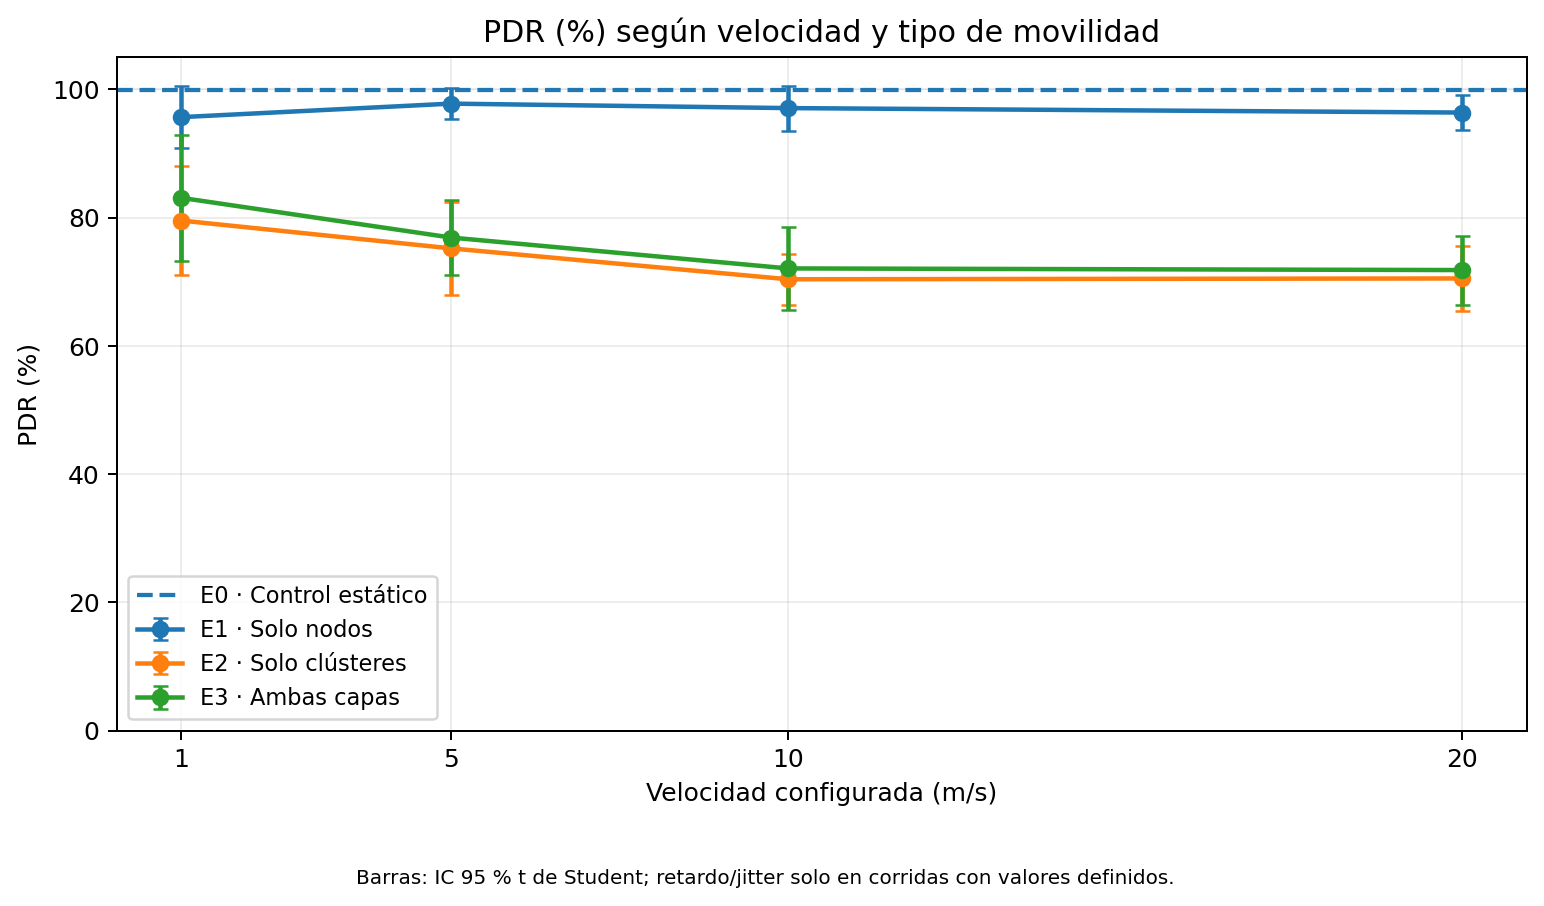
\includegraphics[width=0.75\textwidth]{resultados/figuras/01_pdr_vs_velocidad.png}
\caption{Ejemplo de gráfica generada por \texttt{graficar.py}: PDR contra velocidad
para cada escenario.}
\label{fig:manual-pdr}
\end{figure}

En las gráficas (figura~\ref{fig:manual-pdr}), cada punto es la media de las réplicas
de una configuración y las barras son su intervalo de confianza del 95\,\%. Cuando los
intervalos de dos escenarios no se traslapan, la diferencia entre ellos es clara; cuando
se traslapan, hay que mirar la prueba estadística.

En \texttt{tabla\_\allowbreak{}estadistica.csv}, las columnas que terminan en \texttt{\_\allowbreak{}media},
\texttt{\_\allowbreak{}ic95\_\allowbreak{}inf} y \texttt{\_\allowbreak{}ic95\_\allowbreak{}sup} son la media y los límites del intervalo de
cada métrica, y \texttt{corridas\_\allowbreak{}sin\_\allowbreak{}rx} cuenta las réplicas en las que no llegó
ningún paquete. En esas réplicas el retardo y el \emph{jitter} no se pueden calcular, así
que quedan vacíos en lugar de valer cero.

{\sloppy
En \texttt{comparacion\_\allowbreak{}E2\_\allowbreak{}vs\_\allowbreak{}E1.csv}, cada fila es una velocidad y una métrica. Las
columnas más importantes son \texttt{diferencia\_\allowbreak{}E2\_\allowbreak{}menos\_\allowbreak{}E1}, \texttt{p\_\allowbreak{}unilateral}
y \texttt{rechaza\_\allowbreak{}H0\_\allowbreak{}alpha\_\allowbreak{}0\_\allowbreak{}05}: si esta última vale \texttt{True}, la diferencia
va en la dirección de la hipótesis y es significativa con $\alpha = 0.05$. Según la
regla de decisión del informe (sección «Método de análisis estadístico»), la hipótesis
principal se respalda si eso ocurre en al menos tres de las cuatro velocidades.\par}

\subsection{Visualizar una simulación con NetAnim}

{\sloppy
Con \texttt{-{}-netanim=true}, el programa guarda en la carpeta de salida el archivo
\texttt{netanim\_\allowbreak{}<escenario>\_\allowbreak{}cs<clusterSpeed>\_\allowbreak{}ns<nodeSpeed>\_\allowbreak{}run<RngRun>.xml}. Al
abrirlo con NetAnim, que viene con ns-allinone, se ve el movimiento de los nodos: los CH
en rojo y los miembros en azul.\par}

\subsection{Problemas frecuentes}

\begin{center}
\small
\begin{tabular}{p{5.2cm}p{7.4cm}}
\toprule
\textbf{Mensaje o síntoma} & \textbf{Qué hacer} \\
\midrule
\texttt{No está ./ns3 en ...} o \texttt{No existe el directorio de ns-3} & Indicar la carpeta correcta con \texttt{-{}-ns3} o con la variable \texttt{NS3\_\allowbreak{}DIR}. \\
\texttt{OMITIDO (XML existente)} & Es normal al retomar un experimento. Para repetir esas simulaciones, agregar \texttt{-{}-forzar}. \\
\texttt{ERROR de simulación} & Revisar el archivo de esa simulación en \texttt{resultados/logs/}; el script muestra sus últimas líneas. \\
\texttt{./ns3} no arranca con el Python del sistema & Indicar otro intérprete con la variable \texttt{NS3\_\allowbreak{}PYTHON}. \\
Todo es muy lento en WSL & Mover ns-3 y el repositorio al disco de Linux (\texttt{\textasciitilde}) en vez de \texttt{/mnt/c/...}. \\
\bottomrule
\end{tabular}
\end{center}
